\documentclass{article}
\usepackage{tkz-tab}
\usepackage{amsmath} 
\usepackage{geometry}
\usepackage{indentfirst}
\setlength{\parindent}{-0.5cm} % Retrait du paragraphe
\geometry{
    left=1.5cm }
\begin{document}
TAbleau de variation de $f(x)$\\
                   
$f(x)=- x^{3} + x^{2}$\\
$f'(x)=- 3 x^{2} + 2 x$\\

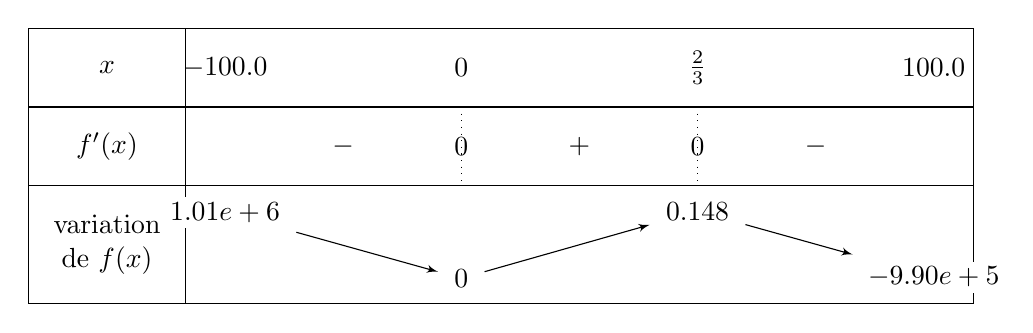
\begin{tikzpicture}
\tkzTabInit[espcl=3]{$x$ / 1 , $f'(x)$ / 1, variation de $f(x)$/1.5}
{$-100.0$,$0$,$\frac{2}{3}$,$100.0$}
\tkzTabLine{,-,z ,+,z ,-}
\tkzTabVar{+/$1.01e+6$,-/$0$,+/$0.148$,-/$-9.90e+5$}
\end{tikzpicture}
\end{document}